\documentclass[tikz,margin=0pt]{standalone}

\usetikzlibrary{shapes, positioning, fadings, backgrounds, intersections, calc, math}

%https://tex.stackexchange.com/questions/179843/make-a-polygon-with-automatically-labelled-nodes-according-to-their-coordinates

\begin{document}


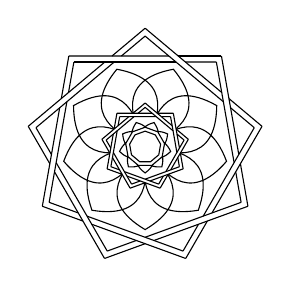
\begin{tikzpicture}

\begin{scope}

\edef\nsides{9}
\pgfmathparse{\nsides-1}\edef\nsidesmin{\pgfmathresult};
 
\def\petal{
  [rounded corners=0] (0,0) %
  .. controls (0.25,0.25) and (0.66,0.66) .. (0,1.05) %
  .. controls (-0.66,0.66) and (-0.25,0.25) .. (0,0) %
}


\def\petalsmall{
  [rounded corners=0] (0,0) %
  .. controls (0.1,0.1) and (0.19,0.19) .. (0,0.33) %
  .. controls (-0.19,0.19) and (-0.1,0.1) .. (0,0) %
}

 
% declare the polygons A is the outer one, and B is the inner one.  
\node[regular polygon, regular polygon sides=\nsides, minimum size=3cm] (A) {};
\node[regular polygon, regular polygon sides=\nsides, minimum size=2.8cm] (B) {};

% Repeat for each edge. 


\foreach \cnt in {0,...,\nsidesmin} {
%%\foreach \i/\j/\p/\q in {1/3/2/4, 3/5/4/6, 5/7/6/8, 7/9/8/1, 9/2/1/3, 2/4/3/5, 4/6/5/7, 6/8/7/9, 8/1/9/2} {
    \pgfmathparse{int(Mod(2*\cnt, \nsides)+1)}\edef\i{\pgfmathresult};
    \pgfmathparse{int(Mod(\i+1, \nsides)+1)}\edef\j{\pgfmathresult};
    \pgfmathparse{int(Mod(\i, \nsides)+1)}\edef\p{\pgfmathresult};
    \pgfmathparse{int(Mod(\i+2, \nsides)+1)}\edef\q{\pgfmathresult};    

    % First identify the four lines.     
    \path [name path=lineE] (A.corner \i) -- (A.corner \j) ;
    \path [name path=lineF] (B.corner \i) -- (B.corner \j);
    \path [name path=lineG] (A.corner \p) -- (A.corner \q);
    \path [name path=lineH] (B.corner \p) -- (B.corner \q);    
    
    % Identify the four intersection points.
    \path [name intersections={of = lineE and lineG, by=IEG}];
    \path [name intersections={of = lineF and lineG, by=IFG}];
    \path [name intersections={of = lineE and lineH, by=IEH}];
    \path [name intersections={of = lineF and lineH, by=IFH}];
    
    % We go below the previous edge, and then it goes above the next edge. 
    \draw [black] (A.corner \p) -- (IEG);
    \draw [black] (IFG) -- (A.corner \q);    
    \draw [black] (B.corner \p) -- (IEH);
    \draw [black] (IFH) -- (B.corner \q); 
}

\pgfmathparse{360/\nsides}\edef\petalangle{\pgfmathresult};
\pgfmathparse{360/\nsides + \petalangle}\edef\petalstephint{\pgfmathresult};
\pgfmathparse{\petalangle/2}\edef\petalangleoffset{\pgfmathresult};
%\edef\petalangleoffset{0}


\foreach \angle in {\petalangle,\petalstephint,...,360} {
    \pgfmathparse{\angle+\petalangleoffset}\edef\thisangle{\pgfmathresult};
    \draw [rotate=\thisangle] \petal; 
}

\node[regular polygon, draw=white, fill=white, regular polygon sides=\nsides, minimum size=0.95cm] {};
\node[regular polygon, regular polygon sides=\nsides, minimum size=1.1cm] (A) {};
\node[regular polygon, regular polygon sides=\nsides, minimum size=0.99cm] (B) {};

\foreach \cnt in {0,...,\nsidesmin} {
%%\foreach \i/\j/\p/\q in {1/3/2/4, 3/5/4/6, 5/7/6/8, 7/9/8/1, 9/2/1/3, 2/4/3/5, 4/6/5/7, 6/8/7/9, 8/1/9/2} {
    \pgfmathparse{int(Mod(2*\cnt, \nsides)+1)}\edef\i{\pgfmathresult};
    \pgfmathparse{int(Mod(\i+1, \nsides)+1)}\edef\j{\pgfmathresult};
    \pgfmathparse{int(Mod(\i, \nsides)+1)}\edef\p{\pgfmathresult};
    \pgfmathparse{int(Mod(\i+2, \nsides)+1)}\edef\q{\pgfmathresult};    

    % First identify the four lines.     
    \path [name path=lineE] (A.corner \i) -- (A.corner \j) ;
    \path [name path=lineF] (B.corner \i) -- (B.corner \j);
    \path [name path=lineG] (A.corner \p) -- (A.corner \q);
    \path [name path=lineH] (B.corner \p) -- (B.corner \q);    
    
    % Identify the four intersection points.
    \path [name intersections={of = lineE and lineG, by=IEG}];
    \path [name intersections={of = lineF and lineG, by=IFG}];
    \path [name intersections={of = lineE and lineH, by=IEH}];
    \path [name intersections={of = lineF and lineH, by=IFH}];
    
    % We go below the previous edge, and then it goes above the next edge. 
    \draw [black] (A.corner \p) -- (IEG);
    \draw [black] (IFG) -- (A.corner \q);    
    \draw [black] (B.corner \p) -- (IEH);
    \draw [black] (IFH) -- (B.corner \q); 
}


\foreach \angle in {\petalangle,\petalstephint,...,360} {
    \pgfmathparse{\angle+\petalangleoffset}\edef\thisangle{\pgfmathresult};
    \draw [rotate=\thisangle] \petalsmall; 
}

%\draw [black, fill=white] (0,0) circle(0.3cm);
%\draw [black, fill=white] (0,0) circle(0.1cm);
\node[regular polygon, draw, fill=white, regular polygon sides=\nsides, minimum size=0.5cm] {};
\node[regular polygon, draw, fill=white, regular polygon sides=\nsides, minimum size=0.4cm] {};

\end{scope}

\end{tikzpicture}

\end{document}
